\documentclass{article}
\usepackage[utf8]{inputenc}
\newcommand{\ii}{{\bf i}}
\newcommand{\jj}{{\bf j}}
\newcommand{\kk}{{\bf k}}
\newcommand{\id}{{\bf 1}}
\newcommand{\hur}{\frac{\id+\ii+\jj+\kk}{2}}%The "Hurwitz point"
\newcommand{\hurwitz}{\Z\left[\hur,\ii,\jj,\kk\right]}%The set of Hurwitz integers
\usepackage{wrapfig}
\usepackage{calligra}
\usepackage[utf8]{inputenc}
\usepackage[dvips]{graphicx}
\usepackage{a4wide}
\usepackage{amsmath}
\usepackage{euscript}
\usepackage{amssymb}
\usepackage{amsthm}
\usepackage{amsopn}
\usepackage[colorinlistoftodos]{todonotes}
\usepackage{graphicx}
\usepackage[T1]{fontenc}
\newcommand\mybar{\kern1pt\rule[-\dp\strutbox]{.8pt}{\baselineskip}\kern1pt}

\usepackage{ulem}
\usepackage{xcolor}
\newcommand{\cs}[1]{\color{blue}{#1}\normalcolor}

%Matrix commands
\newcommand{\ba}{\begin{array}}
\newcommand{\ea}{\end{array}}
\newcommand{\bmat}{\left[\begin{array}}
\newcommand{\emat}{\end{array}\right]}
\newcommand{\bdet}{\left|\begin{array}}
\newcommand{\edet}{\end{array}\right|}
\newcommand{\inv}[1]{#1^{-1}}

%Environment commands
\newcommand{\be}{\begin{enumerate}}
\newcommand{\ee}{\end{enumerate}}
\newcommand{\bi}{\begin{itemize}}
\newcommand{\ei}{\end{itemize}}
\newcommand{\bt}{\begin{thm}}
\newcommand{\et}{\end{thm}}
\newcommand{\bp}{\begin{proof}}
\newcommand{\ep}{\end{proof}}
\newcommand{\bprop}{\begin{prop}}
\newcommand{\eprop}{\end{prop}}
\newcommand{\bl}{\begin{lemma}}
\newcommand{\el}{\end{lemma}}
\newcommand{\bc}{\begin{cor}}
\newcommand{\ec}{\end{cor}}
\newcommand{\lcm}{\mbox{lcm}}
\newcommand{\defn}{\fbox{definition}}
\newcommand{\prop}{\fbox{proposition}}
\newcommand{\stab}{\mbox{stab}}
\newcommand{\Aut}{\mbox{Aut}}
\newcommand{\orb}{\mbox{orb}}

\newcommand{\norm}{\righttriangle}

\newcommand{\and}{\wedge}
\newcommand{\or}{\vee}



%sets of numbers
\newcommand{\N}{\mathbb{N}}
\newcommand{\Z}{\mathbb{Z}}
\newcommand{\Q}{\mathbb{Q}}
\newcommand{\R}{\mathbb{R}}

\newcommand{\topT}{\mathcal{T}}
\newcommand{\standtop}{\mathcal{T}_{STD}}
\newcommand{\cc}{\mathcal{C}}


\title{Topology}
\author{August bergquist}


\begin{document}

\fbox{exercise 3.32} Let $X,Y$ be topological spaces. The \textbf{product topology} on $X\times Y$ is the topology whose basis whose basis is all sets of the form $U\times V$ where $U$ is open in $X$ and $V$ is open in $Y$. Show that this really is a basis.\\

\fbox{proof} To show that this is a basis, we will show that it satisfies the conditions of 3.3. That is, (1) every point in $(a,b)\in X\times Y$ should be in a basic set $U\times V$, and (2) for all basic sets $A\times B$ and $C\times D$, and for every point $p\in (A\times B )\cap (C\times D)$ there is a basic set $W\times Z$ such that $p\in W\times Z \susbeteq (A\times B )\cap (C\times D)$. \\

Let $(a,b)\in X\times Y$ be arbitrary. Then by the cartesian product $a\in X$ and $b\in Y$. Since a topology forms a basis for itself, there is an open set $M$ of $X$ and $N$ of $Y$ such that $a\in M$ and $Y\in N$. Since $N$ and $Y$ are open in their respective spaces, it follows that $(N,M)$ is basic for the product topology. This satisfies requirement (1).\\

Now let $A\times B$ and $C\times D$ be arbitrary basic elements. Let $(p,q)$ be an arbitrary element in $(A\times B)\cap(C\times D)$. Recall from foundations that $(A\times B)\cap (C\times D) = (A\cap C)\times (B\cap D).$ Then by definition of the cartesian product $p\in A\cap C$ and $q\in B\cap D$. Since $A$ and $C$ are elements of the topology on $X$ which is a basis for itself, it follows by theorem 3.3 that there exists a basic (and in this case open in $X$) set $ P$ such that $p\in P\subseteq A\cap C$. There exists a similar open set $Q$ such that $q\in Q\subseteq A\cap C$. Since $p\in P$ and $q\in Q$, both of which are open in their respective spaces, it follows that $p\in P\times Q$, which is open by definition of the basis. Furthermore, recall from foundations that $P\susbeteq (A\cap C)$ and $Q\subseteq (B\cap D)$, it follows that $P\times Q \subseteq (A\cap C) \cap (B\cap D) = (A\times B ) \cap (C\times D).$ Since all of these variables are arbitrary, it applies for all, hence (2) is satisfied.\\

So, by theorem 3.3, we see that this does indeed form the basis for a topology on $X\times Y$.\\


\fbox{exercise 3.3} Draw examples of basic and arbitrary open sets $\R^2 = \R\times \R$ using the standard topology on $\R$. Find an open set in $\R^2$ that is not the product of open sets. Find a closed set in $\R\times \R$ that is not the product of closed sets.\\

These are probably easier to draw on the whiteboard. Here's one exmaple. 

\begin{figure}[htbp]
\centerline{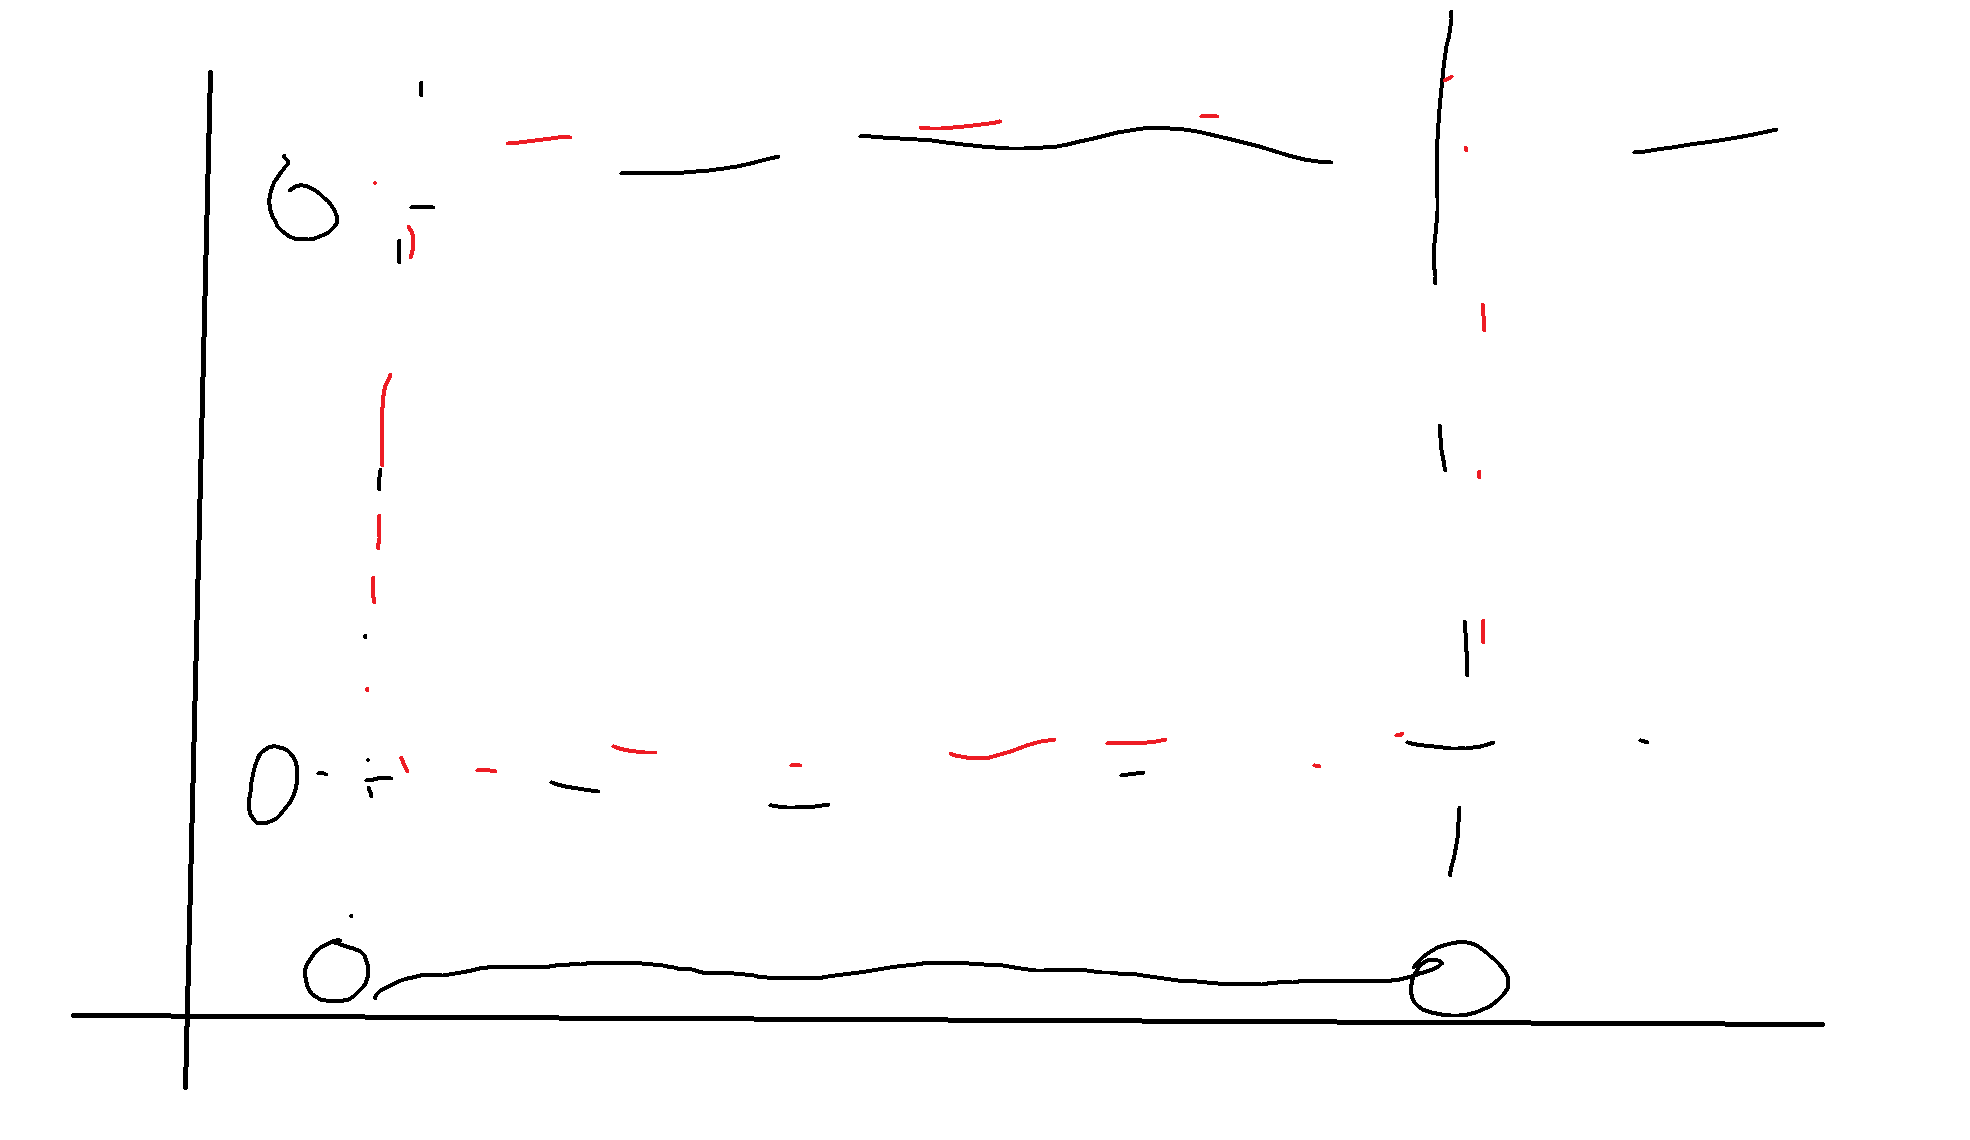
\includegraphics[scale=0.5]{notebook/open_basic.png}}
\caption{other sets are easy to make, draw on whiteboard}
\label{fig}
\end{figure}

For a open set in $\R\times \R$ consider the union of $(1,2)\times(1,2)$ and $(3/2,3)\times (3/2,3)$. This is not the 
\\


\fbox{Theorem 4.1} A space $(X,T)$ is $T_1$ iff every set containing a single point in $X$ is closed. \\

\fbox{proof} Let $p$ be an arbitrary point in the topological space $(X,T)$, and let $(X,T)$ be $T_1$. Suppose that $q$ is a limit point of $\{p\}$. Since the $(X,T)$ is $T_1$, by definition of $T_1$ there exists open set $U$ and $V$ such that $p\in U$ but not in $V$ and $q\in V$ but not in $U$. Since $V$ is an open set containing $q$, it follows by definition of a limit point that $(V-\{q\})\cap \{p\} \ne \emptyset$. Hence there must be something in there, call it $x$. Then $x\in \{p\}$ as well, so $x = p$. Furthermore, by intersection it also follows that $x = p\in V-\{q\}$, hence by set compliment $p\in V$, a contradiction. Hence there are no limit points not in $\{p\}$ so $\{p\}$ is closed.\\


\fbox{4.2} The space $(X,F)$ where $F$ is the finite compliment topology on $X$ is $T_1$.\\

\fbox{proof} Let $p$ and $q$ be distinct points in $(X,F)$. Consider the sets $ U = X-\{q\}$ and $V = X-\{p\}$. Since $X - U = \{q\}$ and $X - V = \{p\}$, both of which are finite, it follows that $U$ and $V$ are open in the finite compliment topology. But by construction and by definition of the set compliment, $U$ and $V$ are open sets such that $q\not\in U$ but $p\in U$ and $p\not\in V$ but $q\in V$. Since $p$ and $q$ are arbitrary, it follows that for any two pairs of points there are empty sets containing one and not the other, and the other and not the one.\\


\fbox{4.3} Show that $\R_{std}$ is $T_2$.\\


\fbox{proof} Consider arbitrary real numbers $ x$ and $y$ such that $y > x$, and consider the open sets $U = (x-1, (y - x)/2)$ and $V = ((y - x)/2, y + 1).$ That is, the open interval from  some point less than $x$ to the middle point between $x$ and $y$, and the middle point between $x$ and $y$ to some point greater than $y$. These two sets are open, contain $x$ and $y$ respectively, and their intersection is empty.

\begin{figure}[htbp]
\centerline{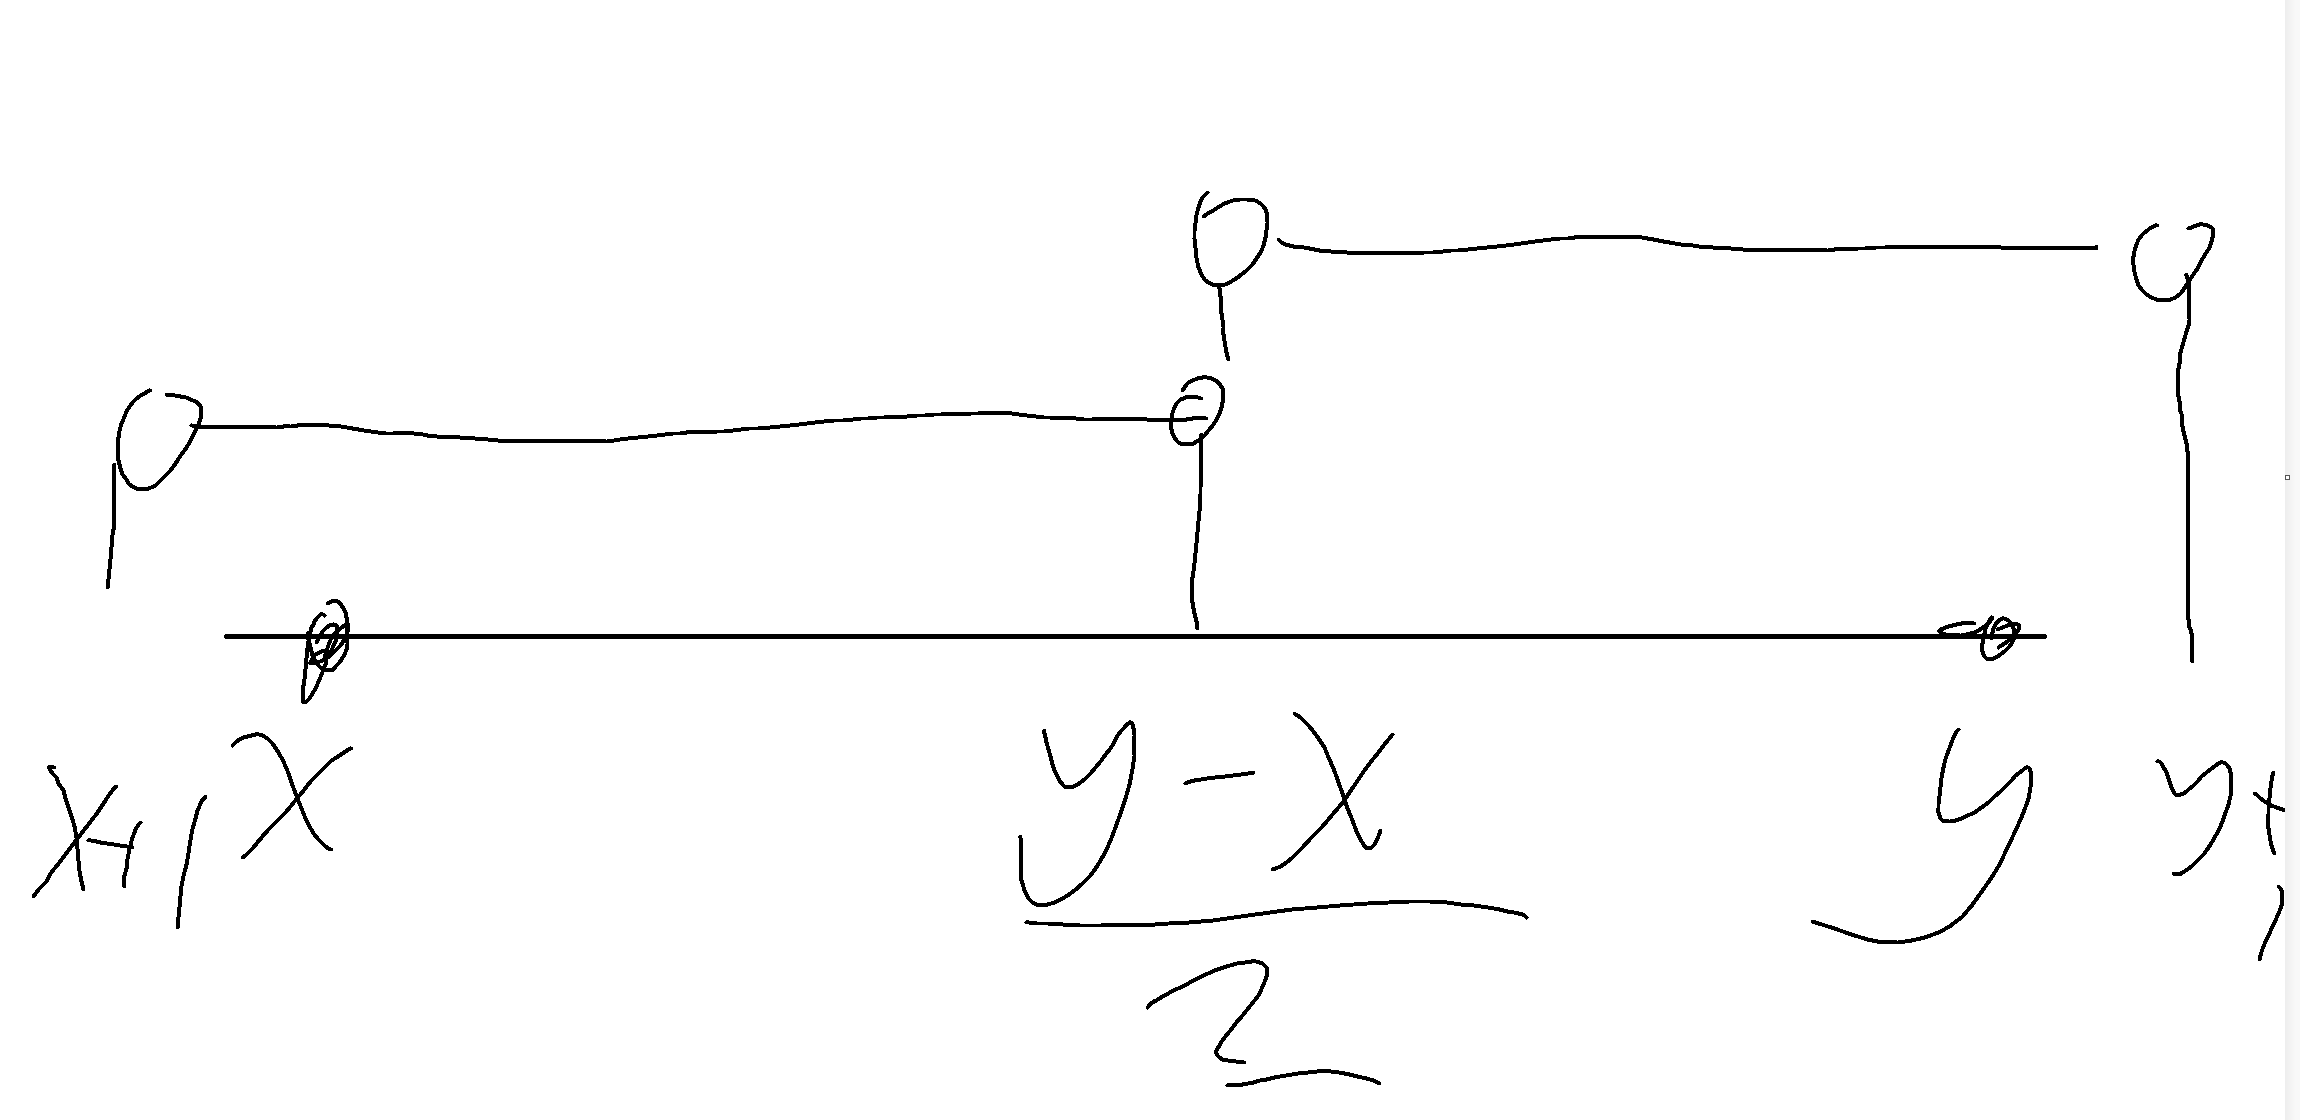
\includegraphics[scale=0.5]{notebook/Screenshot 2022-02-01 214410.png}}
\caption{other sets are easy to make, draw on whiteboard}
\label{fig}
\end{figure}
\end{document}